\documentclass[12pt, letterpaper]{report}
\usepackage{datetime}
\newdateformat{monthyeardate}{\monthname[\THEMONTH] \THEYEAR}

\title{\textbf{ECS 132 Term Project}}
\author{\parbox{\linewidth}{\centering%
  Steven Alvarado, Russell Chien, and Ruth Hailu\endgraf\bigskip
  University of California, Davis}}
\date{\monthyeardate\today}

\usepackage{graphicx} 
\usepackage{titlesec}

\graphicspath{{plots/}}

\titleformat{\chapter}[display]
  {\normalfont\huge\bfseries\filcenter}{\chaptertitlename\ \thechapter}{20pt}{\Huge}
\titlespacing*{\chapter}
  {0pt}{30pt}{20pt}

\begin{document}
\maketitle
\chapter{The Normal Family}
\section{Communities and Crime: pctWWage}

Our group observed that the variable \textbf{pctWWage} of the Communities and Crime dataset seemed well-approximated by the normal family of continuous distributions.
According to the UCI Machine Learning Repository, pctWWage is described as the percentage of households within the United States with wage or salary income in 1989.

\centering
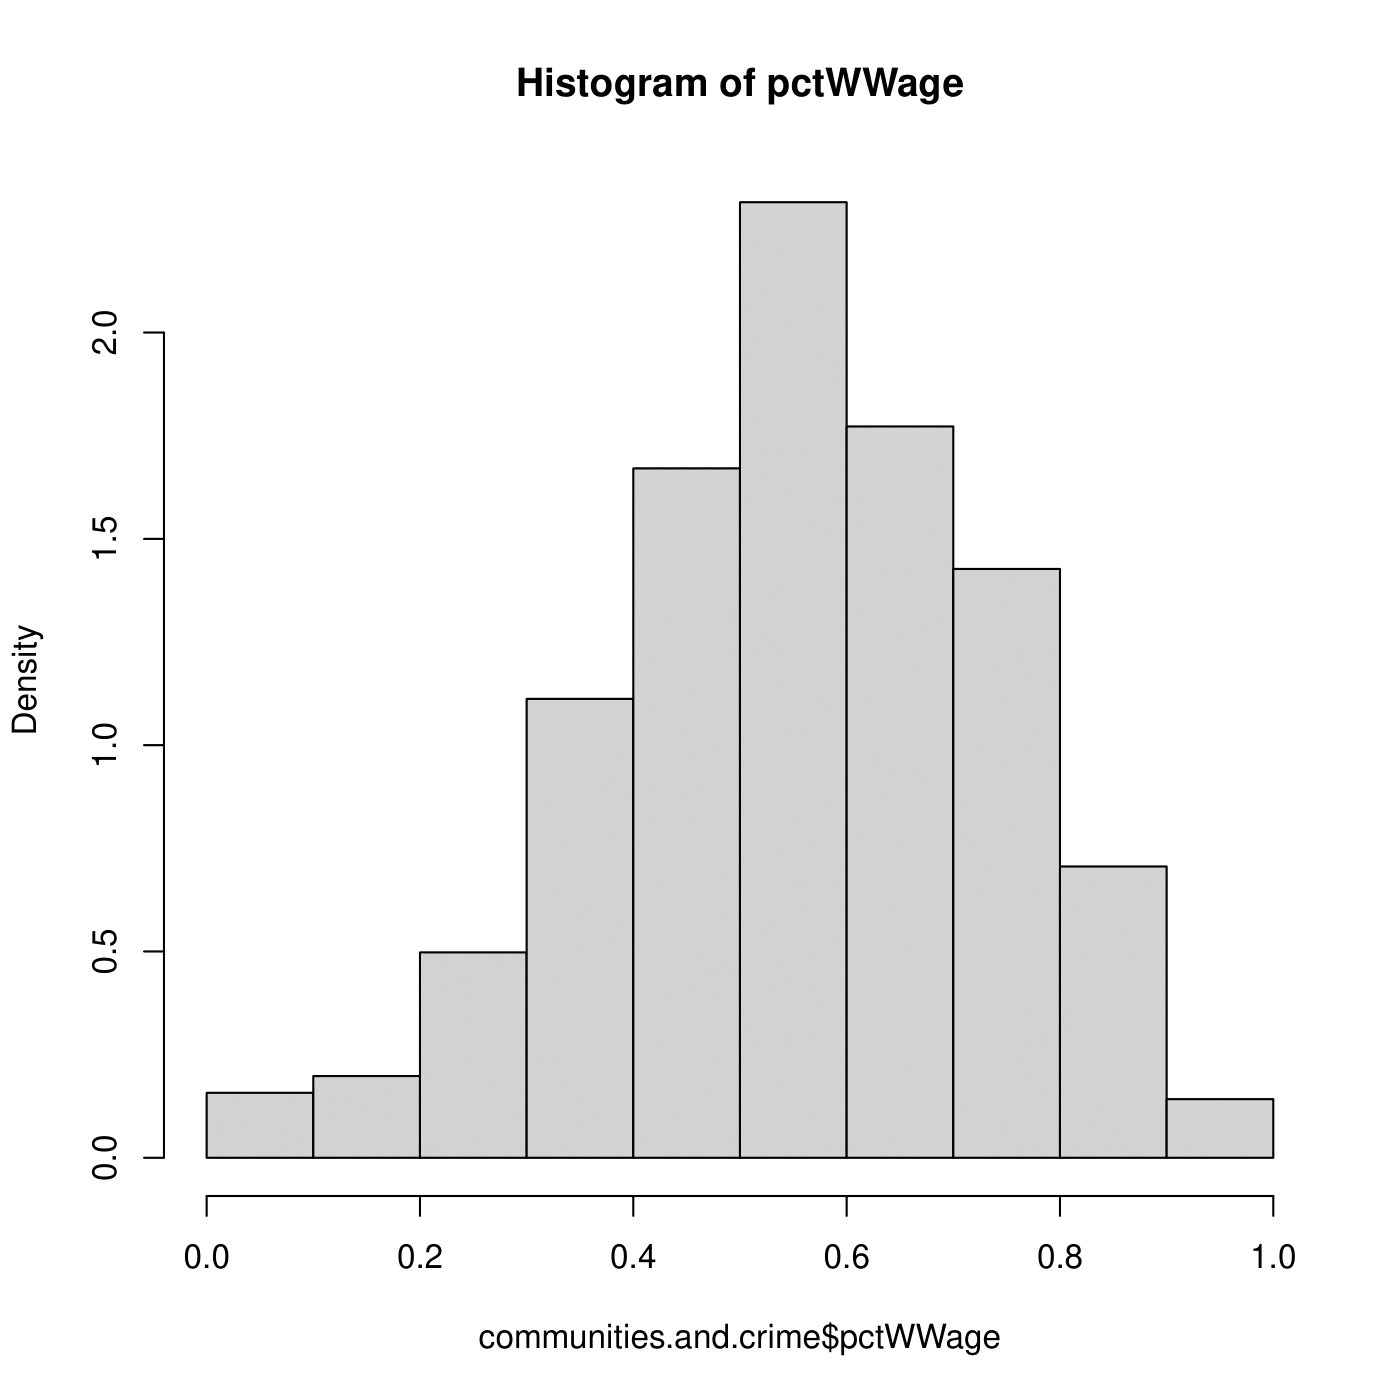
\includegraphics[width=0.45\textwidth]{normal/pctWWage_hist}
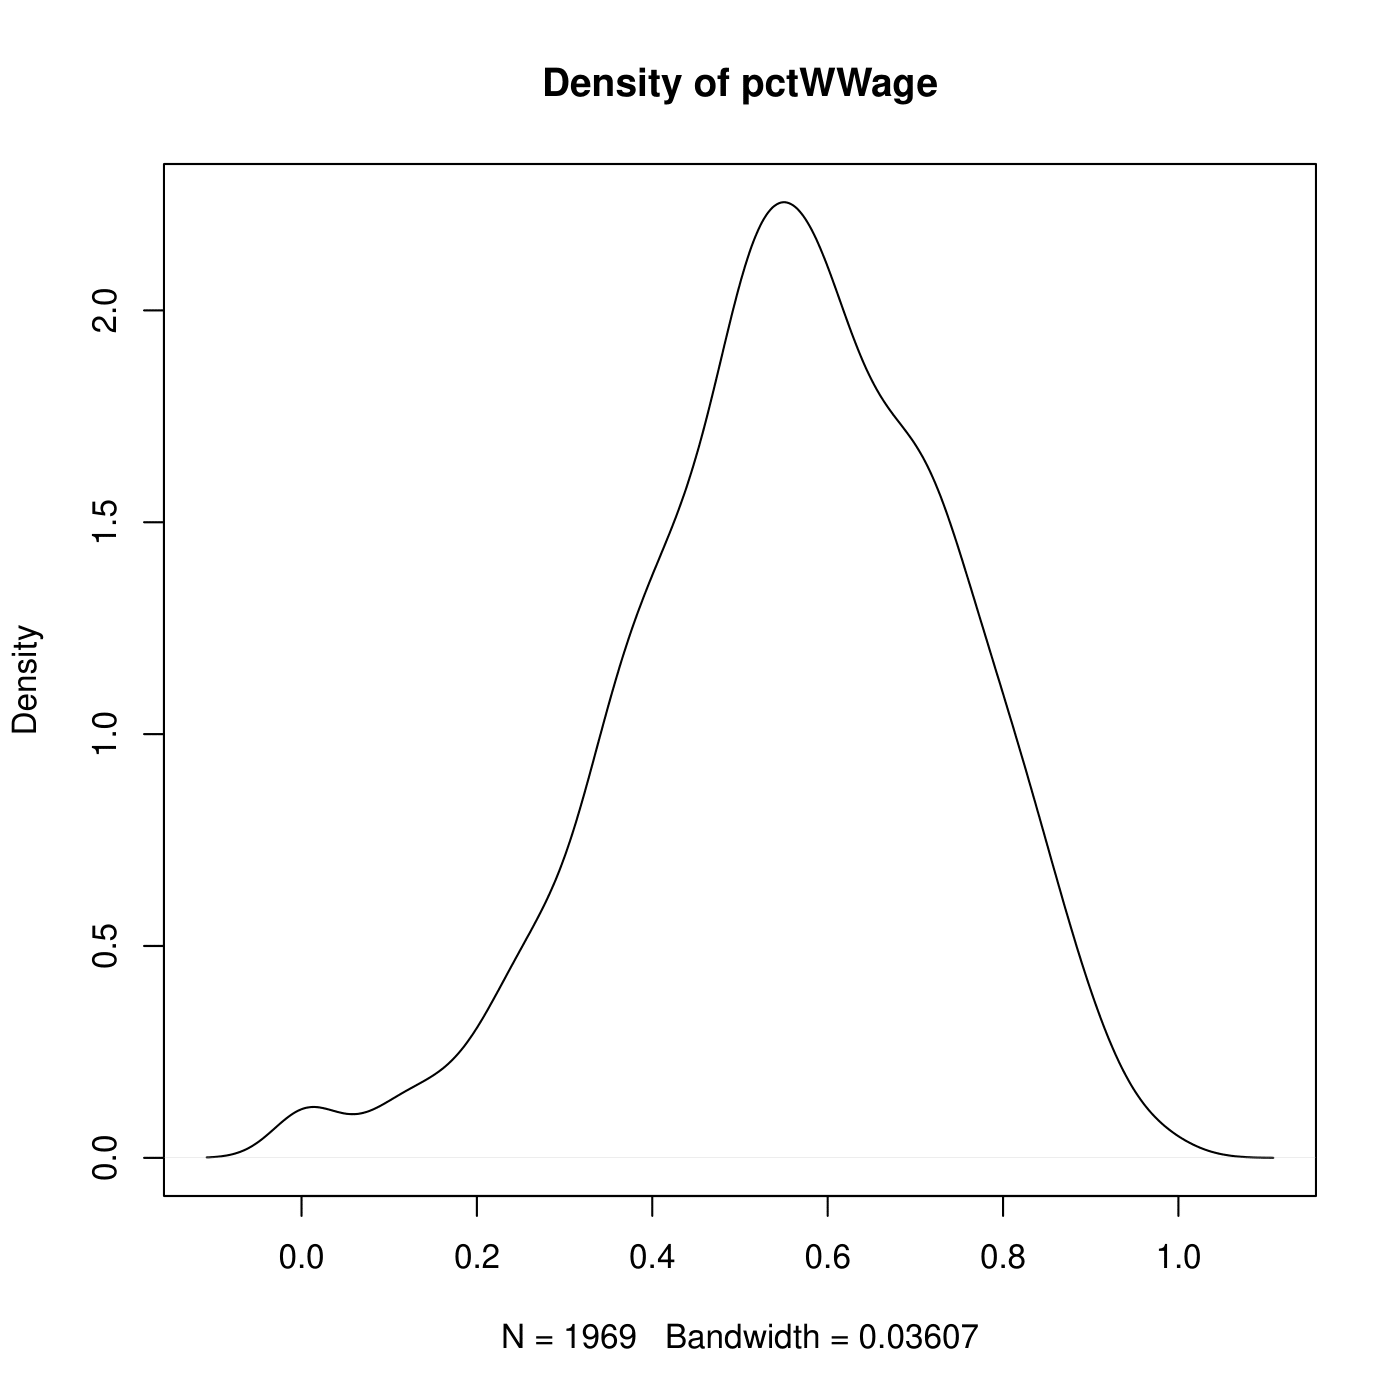
\includegraphics[width=0.45\textwidth]{normal/pctWWage_density}
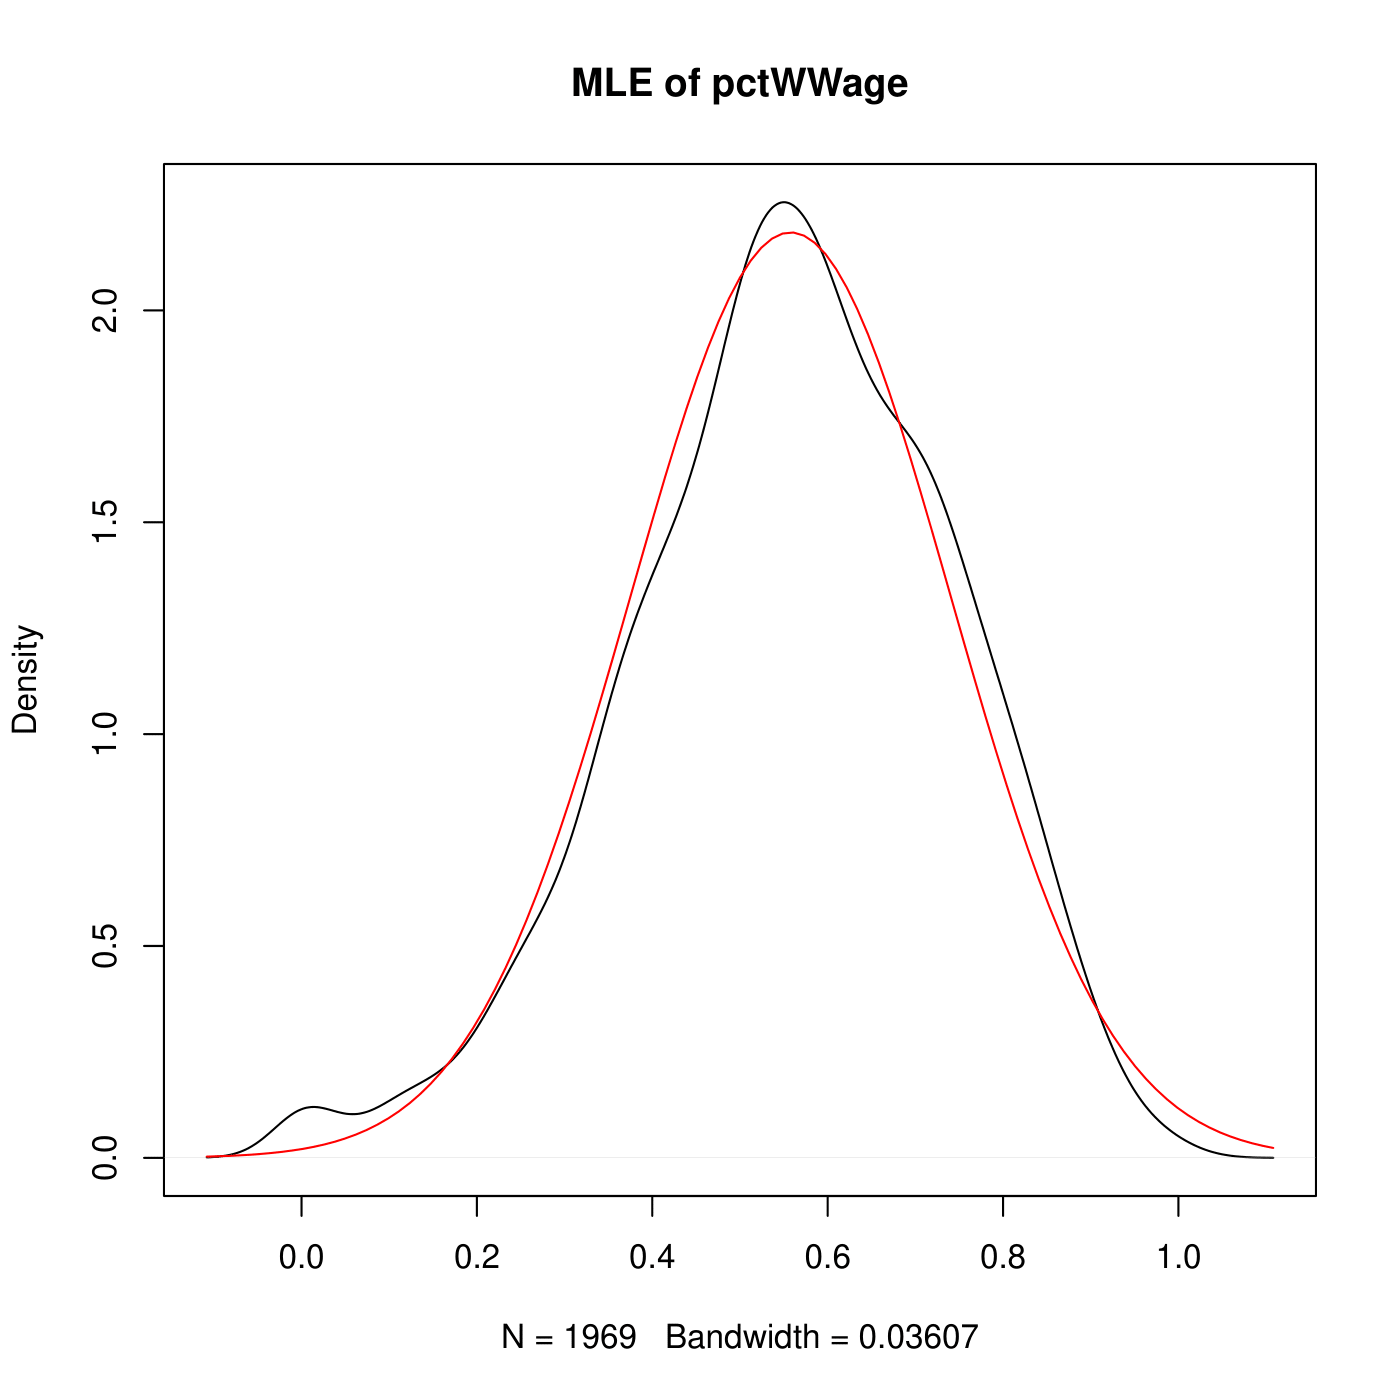
\includegraphics[width=0.45\textwidth]{normal/pctWWage_mle}
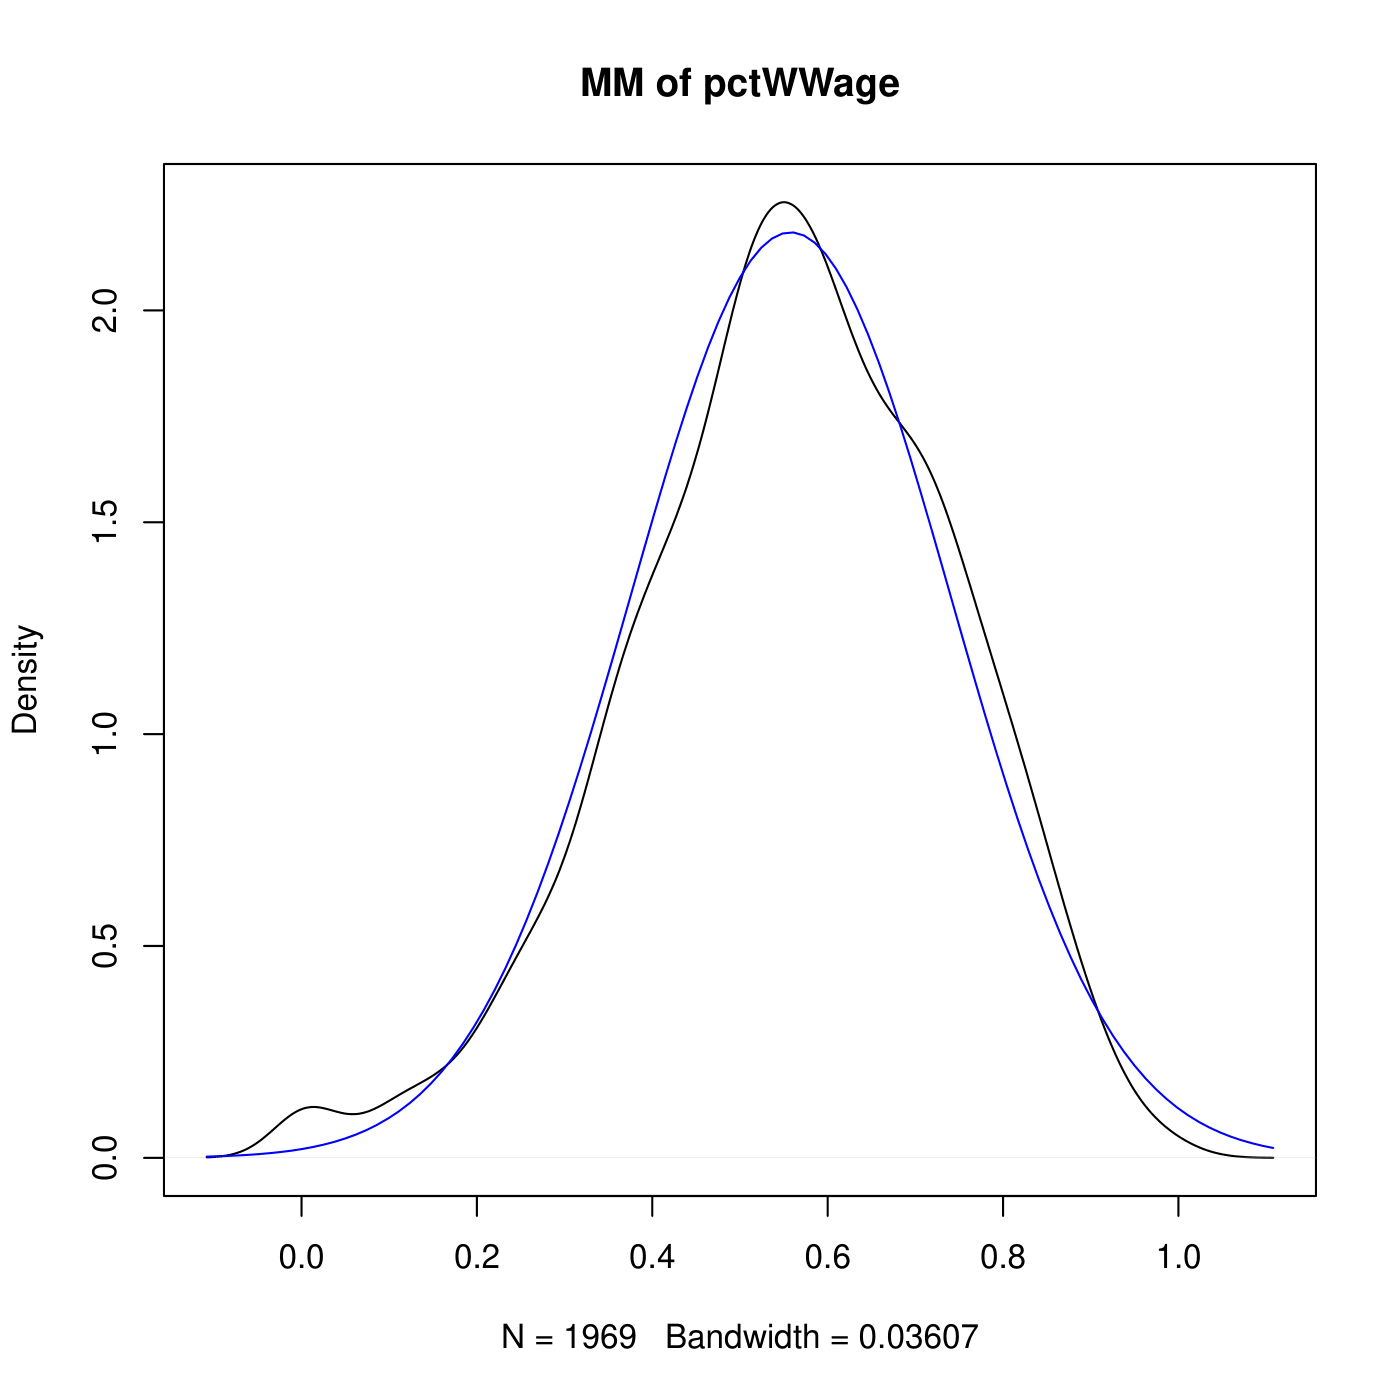
\includegraphics[width=0.45\textwidth]{normal/pctWWage_mm}

\end{document}